\chapter{Fundamental groups}
Topologists can't tell the difference between a coffee cup and a doughnut.
So how do you tell \emph{anything} apart?

This is a very hard question to answer, but one way we can
try to answer it is to find some \emph{invariants} of the space.
To draw on the group analogy, two groups are clearly not isomorphic if,
say, they have different orders, or if one is simple and the other isn't, etc.
We'd like to find some similar properties for topological spaces
so that we can actually tell them apart.

Two such invariants for a space $X$ are
\begin{itemize}
	\ii Defining homology groups $H_1(X)$, $H_2(X)$, \dots
	\ii Defining homotopy groups $\pi_1(X)$, $\pi_2(X)$, \dots
\end{itemize}
Homology groups are hard to define, but in general easier to compute.
Homotopy groups are easier to define but harder to compute.

This chapter is about the fundamental group $\pi_1$.


\section{Fusing paths together}
Recall that a \emph{path} in a space $X$ is a function $[0,1] \to X$.
Suppose we have paths $\gamma_1$ and $\gamma_2$
such that $\gamma_1(1) = \gamma_2(0)$.
We'd like to fuse\footnote{%
	Almost everyone else in the world uses ``gluing'' to describe this
	and other types of constructs.
	But I was traumatized by Elmer's glue when I was in high school
	because I hated the stupid ``make a poster'' projects and hated
	having to use glue on them.
	So I refuse to talk about ``gluing'' paths together, referring
	instead to ``fusing'' them together, which sounds cooler anyways.
} them together to get a path $\gamma_1 \ast \gamma_2$.  Easy, right?

\begin{center}
	\begin{asy}
		size(8cm);
		bigblob("$X$");
		pair A = Drawing("\gamma_1(0)", (-3,-1));
		pair B = Drawing("\gamma_1(1) = \gamma_2(0)", (1,1), dir(90));
		pair C = Drawing("\gamma_2(1)", (2,-2), dir(-90));
		path p = A..(-2,0)..(0,0.5)..B;
		path q = B..(1.8,-0.5)..C;
		draw(p, red, EndArrow);
		draw(q, blue, EndArrow);
		MP("\gamma_1", midpoint(p), dir(90));
		MP("\gamma_2", midpoint(q), dir(0));
	\end{asy}
\end{center}

We unfortunately do have to hack the definition a tiny bit. In an ideal world, we'd have a path $\gamma_1 : [0,1] \to X$ and $\gamma_2 : [1,2] \to X$ and we could just merge them together to get $\gamma_1 \ast \gamma_2 : [0,2] \to X$.
But the ``$2$'' is wrong here.
The solution is that we allocate $[0, \half]$ for the first path
and $[\half, 1]$ for the second path; we run ``twice as fast''.

\begin{definition}
	Given two paths $\gamma_1, \gamma_2 : [0,1] \to X$
	such that $\gamma_1(1) = \gamma_2(0)$, we define
	a path $\gamma_1 \ast \gamma_2 : [0,1] \to X$ by
	\[ 
		(\gamma_1 \ast \gamma_2)(t)
		=
		\begin{cases}
			\gamma_1(2t) & 0 \le t \le \half \\
			\gamma_2(2t-1) & \half \le t \le 1.
		\end{cases}
		\]
\end{definition}

This hack unfortunately reveals a second shortcoming: this ``product'' is not associative.
If we take $(\gamma_1 \ast \gamma_2) \ast \gamma_3$ for some suitable paths,
then $[0, \frac14]$, $[\frac14, \frac12]$ and $[\frac12, 1]$
are the times allocated for $\gamma_1$, $\gamma_2$, $\gamma_3$.
\begin{ques}
	What are the times allocated
	for $\gamma_1 \ast (\gamma_2 \ast \gamma_3)$?
\end{ques}
But I hope you'll agree that even though this operation isn't associative,
the reason it fails to be associative is kind of stupid.
It's just a matter of how fast we run in certain parts.

\begin{center}
	\begin{asy}
		unitsize(6cm);
		D( unitsquare);
		MP("0", (0,0), S);
		MP("1", (1,0), S);
		MP("\frac{1}{4}", (1/4, 0), S);
		MP("\frac{1}{2}", (1/2, 0), S);
		MP("0", (0,1), N);
		MP("1", (1,1), N);
		MP("\frac{3}{4}", (3/4, 1), N);
		MP("\frac{1}{2}", (1/2, 1), N);
		MP("\gamma_1", (1/8, 0), N);
		MP("\gamma_2", (3/8, 0), N);
		MP("\gamma_3", (3/4, 0), N);
		MP("\gamma_1", (1/4, 1), S);
		MP("\gamma_2", (5/8, 1), S);
		MP("\gamma_3", (7/8, 1), S);

		MP("\boxed{\gamma_1 \ast \left( \gamma_2 \ast \gamma_3 \right)}", (0.5,1.2), origin);
		MP("\boxed{\left( \gamma_1 \ast \gamma_2 \right) \ast \gamma_3}", (0.5,-0.2), origin);

		D((1/4,0)--(1/2,1), blue);
		D((1/2,0)--(3/4,1), blue);
		D( (1/2,0)--(1/2,1), dotted);
	\end{asy}
\end{center}

So as long as we're fusing paths together,
we probably don't want to think of $[0,1]$ itself too seriously.
And so we only consider everything up to (path) homotopy equivalence.
(Recall that two paths $\alpha$ and $\beta$ are homotopic if
there's a path homotopy $F : [0,1]^2 \to X$ between them,
which is a continuous deformation from $\alpha$ to $\beta$.)
It is definitely true that
\[
	\left( \gamma_1 \ast \gamma_2 \right) \ast \gamma_3
	\simeq 
	\gamma_1 \ast \left( \gamma_2 \ast \gamma_3 \right) . \]
It is also true that if $\alpha_1 \simeq \alpha_2$ and $\beta_1 \simeq \beta_2$
then $\alpha_1 \ast \beta_1 \simeq \alpha_2 \ast \beta_2$.

Naturally, homotopy is an equivalence relation,
so paths $\gamma$ lives in some ``homotopy type'',
the equivalence classes under $\simeq$. We'll denote this $[\gamma]$.
Then it makes sense to talk about $[\alpha] \ast [\beta]$.
Thus, \textbf{we can think of $\ast$ as an operation on homotopy classes}.


\section{Fundamental groups}
\prototype{$\pi_1(\RR^2)$ is trivial and $\pi_1(S^1) \cong \ZZ$.}

At this point I'm a little annoyed at keeping track of endpoints,
so now I'm going to specialize to a certain type of path.
\begin{definition}
	A \vocab{loop} is a path with $\gamma(0) = \gamma(1)$.
\end{definition}
\begin{center}
	\begin{asy}
		bigblob("$X$");
		pair A = Drawing("x_0", (-1,0), dir(100));
		path p = A..(1,1)..(2,0)..(0.5,-1)..(-1.5,-0.5)..cycle;
		draw(p, blue, EndArrow);
		MP("\gamma", midpoint(p), dir(-20));
	\end{asy}
\end{center}

Hence if we restrict our attention to paths starting at a single point $x_0$,
then we can stop caring about endpoints and start-points, since
everything starts and stops at $x_0$.
We even have a very canonical loop: the ``do-nothing'' loop\footnote{Fatty.} given by standing at $x_0$ the whole time.

\begin{definition}
	Denote the trivial ``do-nothing loop'' by $1$.
	A loop $\gamma$ is \vocab{nulhomotopic} if it is homotopic to $1$; i.e.\ $\gamma \simeq 1$.
\end{definition}

For homotopy of loops, you might visualize ``reeling in'' the loop, contracting it to a single point.

\begin{example}[Loops in $S^2$ are nulhomotopic]
	As the following picture should convince you, every loop in
	the simply connected space $S^2$ is nulhomotopic.
	\begin{center}
		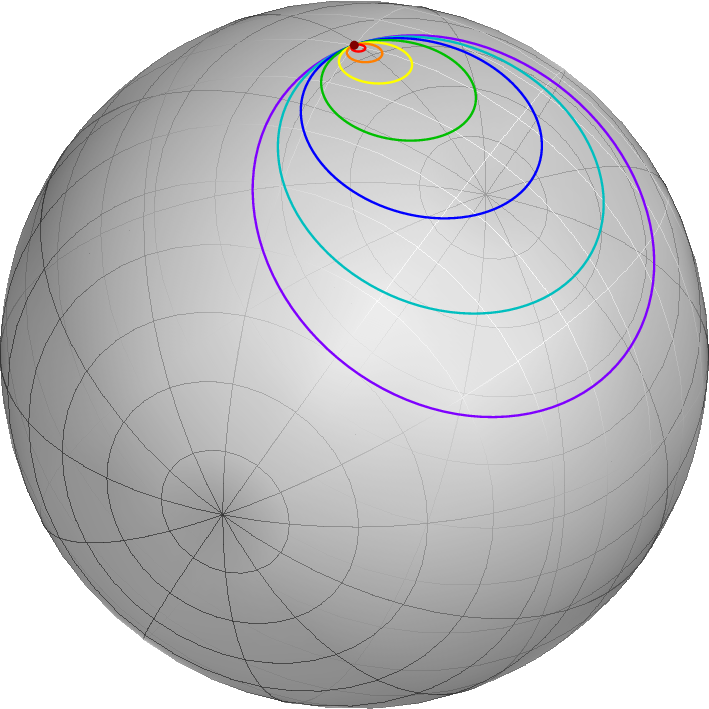
\includegraphics[width=6cm]{media/S2-simply.png}
	\end{center}
	(Starting with the purple loop, we contract to the red-brown point.)
\end{example}

Hence to show that spaces are simply connected it suffices to understand
the loops of that space.
We are now ready to provide:
\begin{definition}
	The \vocab{fundamental group} of $X$ with basepoint $x_0$,
	denoted $\pi_1(X, x_0)$, is the set of homotopy classes
	\[ \left\{ [\gamma] \mid \gamma \text{ a loop at $x_0$} \right\} \]
	equipped with $\ast$ as a group operation.
\end{definition}

It might come as a surprise that this has a group structure.
For example, what is the inverse?
Let's define it now.
\begin{definition}
	Given a path $\alpha : [0,1] \to X$ we can define a path $\ol\alpha$
	\[ \ol\alpha (t) = \alpha(1-t). \]
	In effect, this ``runs $\alpha$ backwards''.
	Note that $\ol\alpha$ starts at the endpoint of $\alpha$
	and ends at the starting point of $\alpha$.
\end{definition}
\begin{exercise}
	Show that for any path $\alpha$,
	$\alpha \ast \ol\alpha$ is homotopic
	to the ``do-nothing'' loop at $\alpha(0)$.
	(Draw a picture.)
\end{exercise}

Let's check it.
\begin{proof}
	[Proof that this is a group structure]
	Clearly $\ast$ takes two loops at $x_0$ and spits out a loop at $x_0$.
	We also already took the time to show that $\ast$ is associative.
	So we only have to check that (i) there's an identity, and (ii)
	there's an inverse.
	\begin{itemize}
		\ii We claim that the identity is the ``do-nothing'' loop $1$
		we described above. The reader can check that for any $\gamma$,
		\[ \gamma \simeq \gamma \ast 1 = 1 \ast \gamma. \]
		\ii For a loop $\gamma$, recall again we define its ``backwards'' loop $\ol\gamma$ by
		\[ \ol\gamma(t) = \gamma(1-t). \]
		Then we have $\gamma \ast \ol\gamma = \ol\gamma \ast \gamma = 1$.
	\end{itemize}
	Hence $\pi_1(X,x_0)$ is actually a group.
\end{proof}

Before going any further I had better give some examples.
\begin{example}
	[Examples of fundamental groups]
	Note that proving the following results is not at all trivial.
	For now, just try to see intuitively why the claimed answer ``should'' be correct.
	\begin{enumerate}[(a)]
		\ii The fundamental group of $\CC$ is the
		trivial group: in the plane, every loop is nulhomotopic.
		(Proof: imagine it's a piece of rope and reel it in.)
		\ii On the other hand, the fundamental group of $\CC - \{0\}$
		(meteor example from earlier) with any base point is actually $\ZZ$!
		We won't be able to prove this for a while,
		but essentially a loop is determined by the number of times
		that it winds around the origin -- these are so-called
		\emph{winding numbers}.  Think about it!
		\ii Similarly, we will soon show that the fundamental group of $S^1$
		(the boundary of the unit circle) is $\ZZ$.
	\end{enumerate}
	Officially, I also have to tell you what the base point is, but
	by symmetry in these examples, it doesn't matter.
\end{example}
Here is the picture for $\CC \setminus \{0\}$, with the hole exaggerated
as the meteor from \Cref{sec:meteor}.
\begin{center}
	\begin{asy}
		size(6cm);
		bigbox("$\mathbb C \setminus \{0\}$");
		filldraw(scale(0.5)*unitcircle, grey, black);
		dot("$x_0$", (1.4,0), dir(0));
		draw( (1.4,0)..(0,1.4)..(-1.4,0)..(1.4*dir(-30))..cycle, blue, EndArrow );
	\end{asy}
\end{center}

\begin{ques}
	Convince yourself that the fundamental group of $S^1$ is $\ZZ$,
	and understand why we call these ``winding numbers''.
	(This will be the most important example of a fundamental group
	in later chapters, so it's crucial you figure it out now.)
\end{ques}

\begin{example}
	[The figure eight]
	\label{ex:figure8}
	Consider a figure eight $S^1 \vee S^1$, and let $x_0$
	be the center.
	Then  \[\pi_1(S^1 \vee S^1, x_0) \cong \left<a,b\right> \]
	is the \emph{free group} generated on two letters.
	The idea is that one loop of the eight is $a$,
	and the other loop is $b$, so we expect $\pi_1$
	to be generated by this loop $a$ and $b$ (and its inverses
	$\ol a$ and $\ol b$).
	These loops don't talk to each other.
	\begin{center}
		\begin{asy}
			draw( shift( (1,0) ) * unitcircle, grey + 5 );
			draw( shift( (-1,0) ) * unitcircle, grey + 5 );
			dot(origin);
			path g = dir(20)..dir(100)..dir(180)..dir(260)..dir(340);
			draw( shift( (1,0) ) * scale(0.8) * reflect(dir(90),dir(-90)) * g, blue, EndArrow );
			draw( shift( (-1,0) ) * scale(0.8) * g, red, EndArrow );
			label("$a$", (-1.6,0), dir(0));
			label("$b$", (1.6,0), dir(180));
		\end{asy}
	\end{center}
\end{example}

Recall that in graph theory, we usually assume our graphs are connected,
since otherwise we can just consider every connected component separately.
Likewise, we generally want to restrict our attention to path-connected spaces, since if a space isn't path-connected then it can be broken into a bunch of ``path-connected components''.
(Can you guess how to define this?)
Indeed, you could imagine a space $X$ that consists of the objects on my desk (but not the desk itself): $\pi_1$ of my phone has nothing to do with $\pi_1$ of my mug. They are just totally disconnected, both figuratively and literally.

But on the other hand we claim that in a path-connected space,
the groups are very related!
\begin{theorem}[Fundamental groups don't depend on basepoint]
	Let $X$ be a path-connected space.
	Then for any $x_1 \in X$ and $x_2 \in X$, we have
	\[ \pi_1(X, x_1) \cong \pi_1(X, x_2). \]
\end{theorem}
Before you read the proof, see if you can guess the isomorphism based just on the picture below.
\begin{center}
	\begin{asy}
		size(7cm);
		bigblob("$X$");
		pair A = Drawing("x_1", (-1.5,0), dir(180));
		pair B = Drawing("x_2", (1.5,0), dir(0));
		draw(A..(-2.5,-0.8)..(-2.5,0.9)..cycle, blue);
		draw(B..(2.2,-1.1)..(2.4,0.8)..cycle, blue);
		draw(A--B, red+dashed, Arrows);
		label("$\alpha$/$\overline{\alpha}$", origin, dir(90));
	\end{asy}
\end{center}
\begin{proof}
	Let $\alpha$ be any path from $x_1$ to $x_2$ (possible by path-connectedness), and let $\ol\alpha$ be its reverse.
	Then we can construct a map
	\[ 
		\pi_1(X,x_1) \to \pi_1(X,x_2)
		\text{ by }
		[\gamma] \mapsto [\ol\alpha \ast \gamma \ast \alpha]. \]
	In other words, given a loop $\gamma$ at $x_1$,
	we can start at $x_2$, follow $\ol\alpha$ to $x_1$,
	run $\gamma$, then run along $\alpha$ home to $x_2$.
	Hence this is a map which builds a loop of $\pi_1(X, x_2)$
	from every loop at $\pi_1(X, x_1)$.
	It is a \emph{homomorphism} of the groups just because
	\[ \left( \ol \alpha \ast \gamma_1 \ast \alpha \right)
		\ast \left( \ol\alpha \ast \gamma_2 \ast \alpha \right)
		= \ol\alpha \ast \gamma_1 \ast \gamma_2 \ast \alpha \]
	as $\alpha \ast \ol\alpha$ is nulhomotopic.

	Similarly, there is a homomorphism
	\[ 
		\pi_1(X,x_2) \to \pi_1(X,x_1)
		\text{ by }
		[\gamma] \mapsto [\alpha \ast \gamma \ast \ol\alpha]. \]
	As these maps are mutual inverses, it follows
	they must be isomorphisms. End of story.
\end{proof}
This is a bigger reason why we usually only care about path-connected spaces.

\begin{abuse}
	For a path-connected space $X$ we will often abbreviate $\pi_1(X, x_0)$
	to just $\pi_1(X)$, since it doesn't matter which $x_0 \in X$
	we pick.
\end{abuse}

Finally, recall that we originally defined ``simply connected'' as saying
that any two paths with matching endpoints were homotopic.
It's possible to weaken this condition and then rephrase it using
fundamental groups.
\begin{exercise}
	Let $X$ be a path-connected space.
	Prove that $X$ is \vocab{simply connected} if and only if
	$\pi_1(X)$ is the trivial group.
	(One direction is easy; the other is a little trickier.)
\end{exercise}
This is the ``usual'' definition of simply connected.


\section{Fundamental groups are functorial}
One quick shorthand I will introduce to clean up the discussion:
\begin{definition}
	By $f : (X, x_0) \to (Y, y_0)$, we will mean that
	$f : X \to Y$ is a continuous function of spaces
	which also sends the point $x_0$ to $y_0$.
\end{definition}

Let $X$ and $Y$ be topological spaces and $f : (X, x_0) \to (Y, y_0)$.
We now want to relate the fundamental groups of $X$ and $Y$.

Recall that a loop $\gamma$ in $(X, x_0)$ is a map $\gamma : [0,1] \to X$
with $\gamma(0) = \gamma(1) = x_0$.
Then if we consider the composition
\[ [0,1] \taking\gamma (X, x_0) \taking f (Y, y_0) \]
then we get straight-away a loop in $Y$ at $y_0$!
Let's call this loop $f_\sharp \gamma$.
\begin{lemma}[$f_\sharp$ is homotopy invariant]
	\label{lem:fsharp_homotopy_invariant}
	If $\gamma_1 \simeq \gamma_2$ are path-homotopic,
	then in fact
	\[ f_\sharp \gamma_1 \simeq f_\sharp \gamma_2. \]
\end{lemma}
\begin{proof}
	Just take the homotopy $h$ taking $\gamma_1$ to $\gamma_2$	
	and consider $f \circ h$.
\end{proof}

It's worth noting at this point that if $X$ and $Y$ are homeomorphic,
then their fundamental groups are all isomorphic.
Indeed, let $f : X \to Y$ and $g : Y \to X$ be mutually inverse continuous maps.
Then one can check that $f_\sharp : \pi_1(X, x_0) \to \pi_1(Y, y_0)$
and $g_\sharp : \pi_1(Y, y_0) \to \pi_1(X, x_0)$ are inverse maps
between the groups (assuming $f(x_0) = y_0$ and $g(y_0) = x_0$).

%Now we want to show that by taking the map $f_\sharp$, we get a \emph{functor}
%\begin{diagram}
%	& (X, x_0) & & \pi_1(X, x_0) & \\
%	\catname{Top}_\ast \ni & \dTo^f & \rDotted & \dTo_{f_\sharp} & \in \catname{Grp} \\
%	& (Y, y_0) & & \pi_1(Y, y_0) &
%\end{diagram}
%\begin{ques}
%	Check this -- we need that $(f \circ g)_\sharp = f_\sharp \circ g_\sharp$
%	and that $(\id_X)_\sharp = \id_{\pi_1(X)}$.
%	Both are totally obvious once you can tell what they're asking.
%\end{ques}
%Thus in this way we've constructed a functor
%\[ \catname{Top}_\ast \to \catname{Grp}. \]
%In particular, by the fact that functors preserve isomorphism (\Cref{thm:functor_isom}), we have
%\begin{moral}
%	Homeomorophic topological spaces have isomorphic fundamental groups.
%	Category theory gives this to us for free.
%\end{moral}
%
%\begin{remark}
%	Note the similarity between this and the construction
%	of the covariant Yoneda functor (\Cref{ex:covariant_yoneda}).
%\end{remark}

\section{Higher homotopy groups}
Why the notation $\pi_1$ for the fundamental group?
And what are $\pi_2$, \dots?
The answer lies in the following rephrasing:
\begin{ques}
	Convince yourself that a loop is the same thing
	as a continuous function $S^1 \to X$.
\end{ques}
It turns out we can define homotopy for things other than paths.
Two functions $f, g : Y \to X$ are \vocab{homotopic} if there exists a continuous
function $Y \times [0,1] \to X$ which continuously deforms $f$ to $g$.
So everything we did above was just the special case $Y = S^1$.

For general $n$, the group $\pi_n(X)$ is defined as the homotopy classes
of the maps $S^n \to X$.
The group operation is a little harder to specify.
You have to show that $S^n$ is homeomorphic to $[0,1]^n$ with
some endpoints fused together; for example $S^1$ is $[0,1]$ with $0$ fused to $1$.
Once you have these cubes, you can merge them together on a face.
(Again, I'm being terribly imprecise, deliberately.)

For $n \neq 1$, $\pi_n$ behaves somewhat differently than $\pi_1$.
(You might not be surprised, as $S^n$ is simply connected for all $n \ge 2$ but not when $n=1$.)
In particular, it turns out that $\pi_n(X)$ is an abelian group for all $n \ge 2$.

Let's see some examples.
\begin{example}[$\pi_n(S^n) \cong \mathbb Z$]
	As we saw, $\pi_1(S^1) \cong \ZZ$; given the base circle $S^1$,
	we can wrap a second circle around it as many times as we want.
	In general, it's true that $\pi_n(S^n) \cong \ZZ$.
\end{example}
\begin{example}[$\pi_n(S^m) \cong \{1\}$ when $n < m$]
	We saw that $\pi_1(S^2) \cong \{1\}$, because 
	a circle in $S^2$ can just be reeled in to a point.
	It turns out that similarly, any smaller $n$-dimensional sphere
	can be reeled in on the surface of a bigger $m$-dimensional sphere.
	So in general, $\pi_n(S^m)$ is trivial for $n < m$.
\end{example}
However, beyond these observations, the groups behave quite weirdly.
Here is a table of $\pi_n(S^m)$ for some values of $m$ and $n$
taken from Wikipedia.

\bgroup
\footnotesize
\[
	\begin{array}{r|rccccccccc}
		\pi_n(S^m) & n = 1 & 2 & 3 & 4 & 5 & 6 & 7 & 8 & 9 & 10 \\ \hline
		m = 1 & \ZZ & \{1\} & \{1\} & \{1\} & \{1\} & \{1\} & \{1\} & \{1\} & \{1\} & \{1\} \\
		2 &  & \ZZ & \ZZ & \Zc2 & \Zc2 & \Zc{12} & \Zc2 & \Zc2 & \Zc3 & \Zc{15}\\
		3 &  &  & \ZZ & \Zc2 & \Zc2 & \Zc{12} & \Zc2 & \Zc2 & \Zc3 & \Zc{15}\\
		4 &  &  &  & \ZZ & \Zc2 & \Zc2 & \ZZ \times \Zc{12} & \Zc2^2 & \Zc2 \times \Zc2 & \Zc{24} \times \Zc3 \\
		5 &  &  &  &  & \ZZ & \Zc2 & \Zc2 & \Zc{24} & \Zc2 & \Zc2 \\
		6 &  &  &  &  &  & \ZZ & \Zc2 & \Zc2 & \Zc{24} & \{1\} \\
		7 &  &  &  &  &  &  & \ZZ & \Zc2 & \Zc2 & \Zc{24} \\
		8 &  &  &  &  &  &  &  & \ZZ & \Zc2 & \Zc2
	\end{array}
\]
\egroup

Actually, it turns out that if you can compute $\pi_n(S^m)$
for every $m$ and $n$,
then you can essentially compute \emph{any} homotopy classes.
Thus, computing $\pi_n(S^m)$ is sort of a lost cause in general,
and the mixture of chaos and pattern in the above table is a testament to this.

\section{Homotopy equivalent spaces}
\prototype{A disk is homotopy equivalent to a point, an annulus is homotopy equivalent to $S^1$.}
Up to now I've abused notation and referred to ``path homotopy'' as just ``homotopy'' for two paths.
I will unfortunately continue to do so (and so any time I say two paths are homotopic, you should assume I mean ``path-homotopic'').
But let me tell you what the general definition of homotopy is first.
\begin{definition}
	Let $f,g : X \to Y$ be continuous functions.
	A \vocab{homotopy} is a continuous function $F : X \times [0,1] \to Y$,
	which we'll write $F_s(x)$ for $s \in [0,1]$, $x \in X$, such that 
	\[ F_0(x) = f(x) \text{ and } F_1(x) = g(x) \text{ for all $x \in X$.} \]
	If such a function exists, then $f$ and $g$ are \vocab{homotopic}.
\end{definition}
Intuitively this is once again ``deforming $f$ to $g$''.
You might notice this is almost exactly the same definition as path-homotopy,
except that $f$ and $g$ are any functions instead of paths, and hence
there's no restriction on keeping some ``endpoints'' fixed through the deformation.

This homotopy can be quite dramatic:
\begin{example}
	The zero function $z \mapsto 0$ and the identity function $z \mapsto z$
	are homotopic as functions $\CC \to \CC$.
	The necessary deformation is
	\[ [0,1] \times \CC \to \CC \text{ by } (t,z) \mapsto tz. \]
\end{example}

I bring this up because I want to define:
\begin{definition}
	Let $X$ and $Y$ be continuous spaces.
	They are \vocab{homotopy equivalent} if there exist
	functions $f : X \to Y$ and $g : Y \to X$ such that
	\begin{enumerate}[(i)]
		\ii $f \circ g : X \to X$ is homotopic to the identity map on $X$, and
		\ii $g \circ f : Y \to Y$ is homotopic to the identity map on $Y$.
	\end{enumerate}
	If a topological space is homotopy equivalent to a point,
	then it is said to be \vocab{contractible}.
\end{definition}
\begin{ques}
	Why are two homeomorphic spaces also homotopy equivalent?
\end{ques}

Intuitively, you can think of this as a more generous form of stretching
and bending than homeomorphism: we are allowed to compress huge spaces into single points.

\begin{example}[$\CC$ is contractible]
	Consider the topological spaces $\CC$
	and the space consisting of the single point $\{0\}$. 
	We claim these spaces are homotopy equivalent (can you guess what $f$ and $g$ are?)
	Indeed, the two things to check are
	\begin{enumerate}[(i)]
		\ii $\CC \to \{0\} \hookrightarrow \CC$ by $z \mapsto 0 \mapsto 0$
		is homotopy equivalent to the identity on $\CC$, which we just saw, and
		\ii $\{0\} \hookrightarrow \CC \to \{0\}$ by $0 \mapsto 0 \mapsto 0$, which \emph{is} the identity on $\{0\}$.
	\end{enumerate}
	Here by $\hookrightarrow$ I just mean $\to$ in the special case
	that the function is just an ``inclusion''.
\end{example}
\begin{remark}
	$\CC$ cannot be \emph{homeomorphic} to a point
	because there is no bijection of sets between them.
\end{remark}

\begin{example}[$\CC \setminus \{0\}$ is homotopy equivalent to $S^1$]
	Consider the topological spaces $\CC \setminus \{0\}$,
	the \vocab{punctured plane}, and the circle $S^1$ viewed as a subset of $S^1$.
	We claim these spaces are actually homotopy equivalent!
	The necessary functions are the inclusion
	\[ S^1 \hookrightarrow \CC \setminus \{0\} \]
	and the function
	\[ \CC \setminus \{0\} \to S^1
		\quad\text{by}\quad
		z \mapsto \frac{z}{\left\lvert z \right\rvert}. \]
	You can check that these satisfy the required condition.
\end{example}
\begin{remark}
	On the other hand, $\CC \setminus \{0\}$ cannot be \emph{homeomorphic} to $S^1$.
	One can make $S^1$ disconnected by deleting two points;
	the same is not true for $\CC \setminus \{0\}$.
\end{remark}
\begin{example}
	[$\text{Disk} = \text{Point}$, $\text{Annulus} = \text{Circle}$.]
	By the same token, a disk is homotopic to a point;
	an annulus is homotopic to a circle.
	(This might be a little easier to visualize, since it's finite.)
\end{example}

I bring these up because it turns out that 
\begin{moral}
	Algebraic topology can't distinguish between homotopy equivalent spaces.
\end{moral}
More precisely,
\begin{theorem}[Homotopy equivalent spaces have isomorphic fundamental groups]
	\label{thm:fundgrp_homotopy_invariant}
	Let $X$ and $Y$ be path-connected, homotopy-equivalent spaces.
	Then $\pi_n(X) \cong \pi_n(Y)$ for every positive integer $n$.
\end{theorem}
\begin{proof}
	Let $\gamma : [0,1] \to X$ be a loop.
	Let $f : X \to Y$ and $g : Y \to X$ be maps witnessing that $X$ and $Y$ are homotopy equivalent
	(meaning $f \circ g$ and $g \circ f$ are each homotopic to the identity).
	Then the composition
	\[ [0,1] \taking\gamma X \taking f Y \]
	is a loop in $Y$ and hence $f$ induces a natural homomorphism $\pi_1(X) \to \pi_1(Y)$.
	Similarly $g$ induces a natural homomorphism $\pi_1(Y) \to \pi_1(X)$.
	The conditions on $f$ and $g$ now say exactly that these two homomorphisms
	are inverse to each other, meaning the maps are isomorphisms.
\end{proof}
In particular,
\begin{ques}
	What are the fundamental groups of contractible spaces?
\end{ques}

That means, for example, that algebraic topology can't tell
the following homotopic subspaces of $\RR^2$ apart.
\begin{center}
	{\color{red} \Huge \venus}
	\qquad
	{\color{blue} \Huge \mars}
\end{center}

\section{The pointed homotopy category}
This section is meant to be read by those who know some basic category theory.
Those of you that don't should come back after reading \Cref{ch:cats,ch:functors}.
Those of you that do will enjoy how succinctly we can summarize
the content of this chapter using categorical notions.

\begin{definition}
	The \vocab{pointed homotopy category} $\catname{hTop}_\ast$ is defined as follows.
	\begin{itemize}
		\ii Objects: pairs $(X, x_0)$ of spaces with a distinguished basepoint, and
		\ii Morphisms: \emph{homotopy classes} of continuous functions $(X, x_0) \to (Y, y_0)$.
	\end{itemize}
\end{definition}
In particular, two path-connected spaces are isomorphic in this category exactly
when they are homotopy equivalent.
Then we can summarize many of the preceding results as follows:
\begin{theorem}[Functorial interpretation of fundamental groups]
	\label{thm:fundgrp_functor}
	There is a functor
	\[ \pi_1 : \catname{hTop}_\ast \to \catname{Grp} \]
	sending
	\begin{diagram}
		(X,x_0) & \rTo & \pi_1(X, x_0) \\
		\dTo^f & & \dTo^{f_\sharp} \\
		(Y,y_0) & \rTo & \pi_1(Y, y_0)
	\end{diagram}
\end{theorem}
This implies several things, like
\begin{itemize}
	\ii The functor bundles the information of $f_\sharp$,
	including the fact that it respects composition.
	In the categorical language, $f_\sharp$ is $\pi_1(f)$.
	\ii Homotopic spaces have isomorphic fundamental group
	(since the spaces are isomorphic in $\catname{hTop}$,
	and functors preserve isomorphism by \Cref{thm:functor_isom}).
	In fact, you'll notice that the proofs
	of \Cref{thm:functor_isom} and \Cref{thm:fundgrp_homotopy_invariant}
	are secretly identical to each other.
	\ii If maps $f, g : (X, x_0) \to (Y, y_0)$ are homotopic,
	then $f_\sharp = g_\sharp$. This is basically \Cref{lem:fsharp_homotopy_invariant}
\end{itemize}

\begin{remark}
	In fact, $\pi_1(X, x_0)$ is the set of arrows $(S^1, 1) \to (X, x_0)$ in $\catname{hTop}_\ast$,
	so this is actually a covariant Yoneda functor (\Cref{ex:covariant_yoneda}),
	except with target $\catname{Grp}$ instead of $\catname{Set}$.
\end{remark}


\section\problemhead

\begin{problem}[Harmonic fan]
	Exhibit a subspace $X$ of the metric space $\RR^2$ which is
	path-connected but for which a point $p$ can be found such that
	any $r$-neighborhood of $p$ with $r < 1$ is not path-connected.
	% harmonic fan
\end{problem}

\begin{dproblem}
	[Special case of Seifert-van Kampen] \gim
	Let $X$ be a topological space.
	Suppose $U$ and $V$ are connected open subsets of $X$, with $X = U \cup V$,
	so that $U \cap V$ is nonempty and path-connected.
		
	Prove that if $\pi_1(U) = \pi_1(V) = \{1\}$ then $\pi_1(X) = 1$.
\end{dproblem}
\begin{remark}
	The \vocab{Seifert--van Kampen theorem} generalizes this 
	for $\pi_1(U)$ and $\pi_1(V)$ any groups; it gives a formula for calculating $\pi_1(X)$
	in terms of $\pi_1(U)$, $\pi_1(V)$, $\pi_1(U \cap V)$.
	The proof is much the same.
	
	Unfortunately, this does not give us a way to calculate $\pi_1(S^1)$,
	because it is not possible to write $S^1 = U \cup V$ for $U \cap V$ \emph{connected}.
\end{remark}

\begin{problem}
	[RMM 2013] \yod
	Let $n \ge 2$ be a positive integer.
	A stone is placed at each vertex of a regular $2n$-gon.
	A move consists of selecting an edge of the $2n$-gon and swapping the two stones at the endpoints of the edge.
	Prove that if a sequence of moves swaps every pair of stones exactly once, then there is some edge never used in any move.
\end{problem}
(This last problem doesn't technically have anything to do with the chapter,
but the ``gut feeling'' which motivates the solution is very similar.)
